% Options for packages loaded elsewhere
\PassOptionsToPackage{unicode}{hyperref}
\PassOptionsToPackage{hyphens}{url}
%
\documentclass[
  10pt,
  letterpaper,
  DIV=11,
  numbers=noendperiod,
  twoside]{scrartcl}

\usepackage{amsmath,amssymb}
\usepackage{setspace}
\usepackage{iftex}
\ifPDFTeX
  \usepackage[T1]{fontenc}
  \usepackage[utf8]{inputenc}
  \usepackage{textcomp} % provide euro and other symbols
\else % if luatex or xetex
  \usepackage{unicode-math}
  \defaultfontfeatures{Scale=MatchLowercase}
  \defaultfontfeatures[\rmfamily]{Ligatures=TeX,Scale=1}
\fi
\usepackage{lmodern}
\ifPDFTeX\else  
    % xetex/luatex font selection
  \setmainfont[ItalicFont=EB Garamond Italic,BoldFont=EB Garamond
Bold]{EB Garamond Math}
  \setsansfont[]{Europa-Bold}
  \setmathfont[]{Garamond-Math}
\fi
% Use upquote if available, for straight quotes in verbatim environments
\IfFileExists{upquote.sty}{\usepackage{upquote}}{}
\IfFileExists{microtype.sty}{% use microtype if available
  \usepackage[]{microtype}
  \UseMicrotypeSet[protrusion]{basicmath} % disable protrusion for tt fonts
}{}
\usepackage{xcolor}
\usepackage[left=1in, right=1in, top=0.8in, bottom=0.8in,
paperheight=9.5in, paperwidth=6.5in, includemp=TRUE, marginparwidth=0in,
marginparsep=0in]{geometry}
\setlength{\emergencystretch}{3em} % prevent overfull lines
\setcounter{secnumdepth}{3}
% Make \paragraph and \subparagraph free-standing
\ifx\paragraph\undefined\else
  \let\oldparagraph\paragraph
  \renewcommand{\paragraph}[1]{\oldparagraph{#1}\mbox{}}
\fi
\ifx\subparagraph\undefined\else
  \let\oldsubparagraph\subparagraph
  \renewcommand{\subparagraph}[1]{\oldsubparagraph{#1}\mbox{}}
\fi


\providecommand{\tightlist}{%
  \setlength{\itemsep}{0pt}\setlength{\parskip}{0pt}}\usepackage{longtable,booktabs,array}
\usepackage{calc} % for calculating minipage widths
% Correct order of tables after \paragraph or \subparagraph
\usepackage{etoolbox}
\makeatletter
\patchcmd\longtable{\par}{\if@noskipsec\mbox{}\fi\par}{}{}
\makeatother
% Allow footnotes in longtable head/foot
\IfFileExists{footnotehyper.sty}{\usepackage{footnotehyper}}{\usepackage{footnote}}
\makesavenoteenv{longtable}
\usepackage{graphicx}
\makeatletter
\def\maxwidth{\ifdim\Gin@nat@width>\linewidth\linewidth\else\Gin@nat@width\fi}
\def\maxheight{\ifdim\Gin@nat@height>\textheight\textheight\else\Gin@nat@height\fi}
\makeatother
% Scale images if necessary, so that they will not overflow the page
% margins by default, and it is still possible to overwrite the defaults
% using explicit options in \includegraphics[width, height, ...]{}
\setkeys{Gin}{width=\maxwidth,height=\maxheight,keepaspectratio}
% Set default figure placement to htbp
\makeatletter
\def\fps@figure{htbp}
\makeatother
% definitions for citeproc citations
\NewDocumentCommand\citeproctext{}{}
\NewDocumentCommand\citeproc{mm}{%
  \begingroup\def\citeproctext{#2}\cite{#1}\endgroup}
\makeatletter
 % allow citations to break across lines
 \let\@cite@ofmt\@firstofone
 % avoid brackets around text for \cite:
 \def\@biblabel#1{}
 \def\@cite#1#2{{#1\if@tempswa , #2\fi}}
\makeatother
\newlength{\cslhangindent}
\setlength{\cslhangindent}{1.5em}
\newlength{\csllabelwidth}
\setlength{\csllabelwidth}{3em}
\newenvironment{CSLReferences}[2] % #1 hanging-indent, #2 entry-spacing
 {\begin{list}{}{%
  \setlength{\itemindent}{0pt}
  \setlength{\leftmargin}{0pt}
  \setlength{\parsep}{0pt}
  % turn on hanging indent if param 1 is 1
  \ifodd #1
   \setlength{\leftmargin}{\cslhangindent}
   \setlength{\itemindent}{-1\cslhangindent}
  \fi
  % set entry spacing
  \setlength{\itemsep}{#2\baselineskip}}}
 {\end{list}}
\usepackage{calc}
\newcommand{\CSLBlock}[1]{\hfill\break\parbox[t]{\linewidth}{\strut\ignorespaces#1\strut}}
\newcommand{\CSLLeftMargin}[1]{\parbox[t]{\csllabelwidth}{\strut#1\strut}}
\newcommand{\CSLRightInline}[1]{\parbox[t]{\linewidth - \csllabelwidth}{\strut#1\strut}}
\newcommand{\CSLIndent}[1]{\hspace{\cslhangindent}#1}

\setlength\heavyrulewidth{0ex}
\setlength\lightrulewidth{0ex}
\usepackage[automark]{scrlayer-scrpage}
\clearpairofpagestyles
\cehead{
  Brian Weatherson
  }
\cohead{
  Four Problems in Decision Theory
  }
\ohead{\bfseries \pagemark}
\cfoot{}
\makeatletter
\newcommand*\NoIndentAfterEnv[1]{%
  \AfterEndEnvironment{#1}{\par\@afterindentfalse\@afterheading}}
\makeatother
\NoIndentAfterEnv{itemize}
\NoIndentAfterEnv{enumerate}
\NoIndentAfterEnv{description}
\NoIndentAfterEnv{quote}
\NoIndentAfterEnv{equation}
\NoIndentAfterEnv{longtable}
\NoIndentAfterEnv{abstract}
\renewenvironment{abstract}
 {\vspace{-1.25cm}
 \quotation\small\noindent\rule{\linewidth}{.5pt}\par\smallskip
 \noindent }
 {\par\noindent\rule{\linewidth}{.5pt}\endquotation}
\KOMAoption{captions}{tableheading}
\makeatletter
\@ifpackageloaded{caption}{}{\usepackage{caption}}
\AtBeginDocument{%
\ifdefined\contentsname
  \renewcommand*\contentsname{Table of contents}
\else
  \newcommand\contentsname{Table of contents}
\fi
\ifdefined\listfigurename
  \renewcommand*\listfigurename{List of Figures}
\else
  \newcommand\listfigurename{List of Figures}
\fi
\ifdefined\listtablename
  \renewcommand*\listtablename{List of Tables}
\else
  \newcommand\listtablename{List of Tables}
\fi
\ifdefined\figurename
  \renewcommand*\figurename{Figure}
\else
  \newcommand\figurename{Figure}
\fi
\ifdefined\tablename
  \renewcommand*\tablename{Table}
\else
  \newcommand\tablename{Table}
\fi
}
\@ifpackageloaded{float}{}{\usepackage{float}}
\floatstyle{ruled}
\@ifundefined{c@chapter}{\newfloat{codelisting}{h}{lop}}{\newfloat{codelisting}{h}{lop}[chapter]}
\floatname{codelisting}{Listing}
\newcommand*\listoflistings{\listof{codelisting}{List of Listings}}
\makeatother
\makeatletter
\makeatother
\makeatletter
\@ifpackageloaded{caption}{}{\usepackage{caption}}
\@ifpackageloaded{subcaption}{}{\usepackage{subcaption}}
\makeatother
\ifLuaTeX
  \usepackage{selnolig}  % disable illegal ligatures
\fi
\IfFileExists{bookmark.sty}{\usepackage{bookmark}}{\usepackage{hyperref}}
\IfFileExists{xurl.sty}{\usepackage{xurl}}{} % add URL line breaks if available
\urlstyle{same} % disable monospaced font for URLs
\hypersetup{
  pdftitle={Four Problems in Decision Theory},
  pdfauthor={Brian Weatherson},
  hidelinks,
  pdfcreator={LaTeX via pandoc}}

\title{Four Problems in Decision Theory}
\author{Brian Weatherson}
\date{2024}

\begin{document}
\maketitle
\begin{abstract}
In recent years the literature on decision theory has become disjointed.
There isn't as much discussion as there should be on how different
problems impact one another. This paper aims to bring together work on
problems involving demons, problems about attitudes to risk, problems
about incomplete preferences, and problems about dynamic choice. In the
first three of these cases, I end up defending a pre-existing view. I
defend a ratificationist approach to problems with demons, the orthodox
expected utility approach to risk, and the permissibility of incomplete
preferences. These views are familiar, but seeing how they are related
to a common strengthens the case for each of them. The most novel part
of the view is the theory of dynamic choice that I offer: a sequence of
choices is rational only if both the so-called `resolute' and
`sophisticated' theories of dynamic choice would permit it. This theory
would be implausible if paired with many rival solutions to the first
three problems, but fits nicely with the view I'll develop through the
paper.
\end{abstract}

\setstretch{1.1}
Contemporary decision theory has become disjointed. There is less
overlap than there should be in work on adjacent problems. This paper
aims to undo some of that, by showing that four problems that have
largely been worked on in isolation cast useful light on each other. In
particular, I'll argue that we can go a long way towards solving all
four problems by working through the consequences of a plausible
principle that I'll call the Single Choice Principle.

The Single Choice Principle (hereafter, SCP) relates theories of static
choice and dynamic choice. In particular, it says that for a narrow
class of games, it doesn't matter whether you think of the game as
involving a static, strategic choice, or a dynamic choice that is made
during a game. One way into the principle is to think about an oddity in
the way Newcomb's Problem is normally introduced.

\section{Newcomb's Problem}\label{sec-newcomb}

\subsection{Standard Version}\label{sec-newcomb-standard}

In the standard vignette that goes with Newcomb's Problem, it is a
dynamic game. The demon makes a \emph{prediction}, and then the human
(hereafter, Chooser) makes a choice. Chooser doesn't know what Demon
did, but they do know that Demon has acted. So the natural presentation
of Newcomb's Problem is in a tree like
Figure~\ref{fig-standard-newcomb}.\footnote{I'll assume \$1,000 is worth
  1 util. I think this assumption of constant marginal utility is close
  to incoherent, and it will get relaxed later, but it's harmless for
  now.}

\subsection{Tree}

\begin{figure}

\centering{

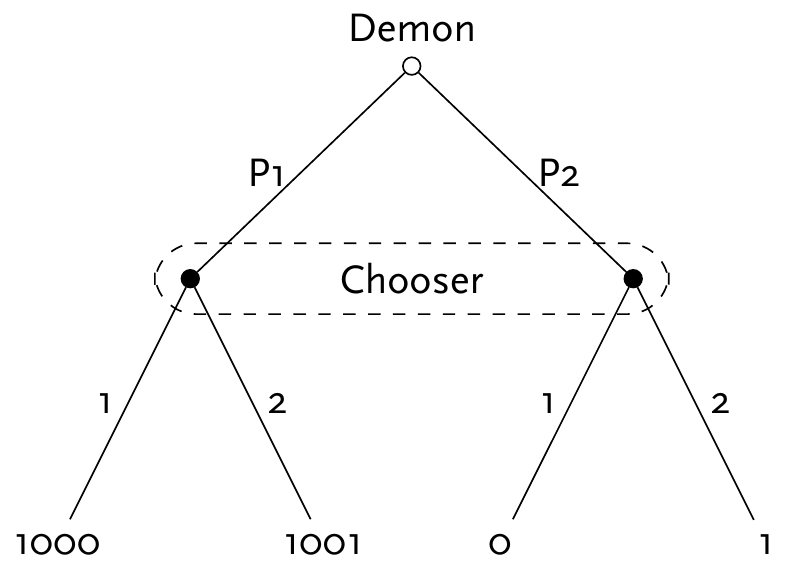
\includegraphics{four-problems-may-19-2024_files/figure-pdf/fig-standard-newcomb-1.png}

}

\caption{\label{fig-standard-newcomb}Newcomb's Problem.}

\end{figure}%

\subsection{Table}

\begin{longtable}[]{@{}ccc@{}}
\caption{Newcomb's Problem}\label{tbl-standard-newcomb}\tabularnewline
\toprule\noalign{}
& P1 & P2 \\
\midrule\noalign{}
\endfirsthead
\toprule\noalign{}
& P1 & P2 \\
\midrule\noalign{}
\endhead
\bottomrule\noalign{}
\endlastfoot
1 & 1000 & 0 \\
2 & 1001 & 1 \\
\end{longtable}

I'll go over the details of how to read diagrams like
Figure~\ref{fig-standard-newcomb} in \textbf{?@sec-dualmandate}. All you
need to know for now is that the game starts at the open node, here at
the top, and it moves along by the agent (Demon or Chooser) making
choices. The dotted lines around the two nodes where Chooser acts mean
that those two nodes are in the same \textbf{information set}. That is,
when Chooser is at either one of those nodes, the strongest thing
Chooser knows is that they are somewhere or other in the set.\footnote{This
  formalism only really makes sense if we presuppose the right epistemic
  logic is S5, and there are good reasons to not make that assumption in
  general (\citeproc{ref-Humberstone2016}{Humberstone 2016, 380--402}).
  For this paper we'll treat it as a simplifying assumption that really
  should be relaxed in subsequent work.} So this tree represents the
standard vignette for Newcomb's Problem. Demon makes a prediction - I'm
in general using PX for Demon predicting X - and Chooser knows that the
prediction has been made, and that either P1 or P2 happened, but chooses
without knowing which it is. Then the game is resolved.

What Table~\ref{tbl-standard-newcomb} shows is a subtly different story.
In Table~\ref{tbl-standard-newcomb}, each player chooses a
\emph{strategy}. A strategy for a player in a tree like
Figure~\ref{fig-standard-newcomb} is a decision about what to do at each
node in the tree where that player has to move.\footnote{In game theory,
  it is usually specified that strategies include decisions about what
  to do at nodes that are ruled out by earlier moves in that very
  strategy. In theory I'm assuming this whenever I talk about
  strategies; in practice it doesn't matter for any application in this
  paper.} So what Table~\ref{tbl-standard-newcomb} represents is a
situation where each player chooses a strategy simultaneously, and that
determines a result for the game. It differs from
Figure~\ref{fig-standard-newcomb} in part in that it's symmetric; there
is no hint that Demon moves first.

There is a lot of disagreement about Newcomb's Problem, but here is one
point of universal agreement: Figure~\ref{fig-standard-newcomb} and
Table~\ref{tbl-standard-newcomb} have the same solutions. It would be
incoherent to prefer taking 1 box in one of these puzzles and 2 boxes in
the other, or to say that both options were choice-worthy in one puzzle
but not the other. They may not represent exactly the same problem, they
don't pose exactly the same question to Chooser, but they should get the
same answer (or answers).

I'm going to agree with the unanimous verdict on this point, but I'll
start dissenting from orthodox opinion very soon. And one way into my
dissent is to ask, why should Figure~\ref{fig-standard-newcomb} and
Table~\ref{tbl-standard-newcomb} get the same answer? What principle is
someone who gives different answers to the two questions violating? I
have a suggestion for what principle that might be, the SCP, but to make
that suggestion plausible we need a couple more examples.

\subsection{Variant 1: Coin-then-Demon}\label{variant-1-coin-then-demon}

Consider a variant on Newcomb's Problem I'll call Coin-Then-Demon. In
this game a fair coin will be flipped and shown to Demon and Chooser. If
it lands Heads, Chooser will get \$5,000 and the game ends. Otherwise,
they play standard Newcomb Problem. Figure~\ref{fig-coin-then-demon}
shows the game tree for this game, with Nature moving first, and the
probabilities of Nature's moves shown. And
Table~\ref{tbl-coin-then-demon} shows the strategy table for it, with
the payouts shown in expected value.\footnote{I will drop the assumption
  that Chooser maximises expected value in Section~\ref{sec-buchak}, but
  it's a harmless assumption for now.}

\subsection{Tree}

\begin{figure}

\centering{

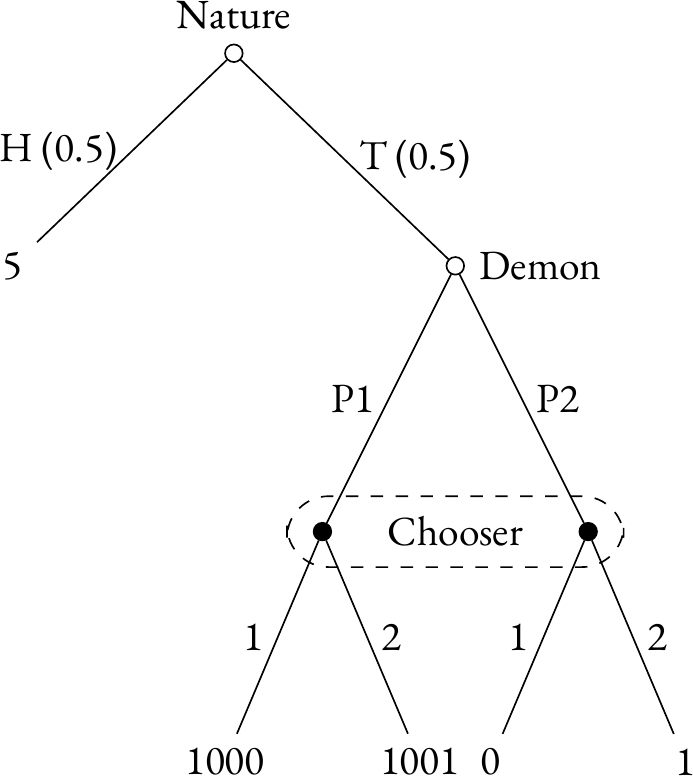
\includegraphics{four-problems-may-19-2024_files/figure-pdf/fig-coin-then-demon-1.png}

}

\caption{\label{fig-coin-then-demon}Coin-then-Demon}

\end{figure}%

\subsection{Table}

\begin{longtable}[]{@{}ccc@{}}
\caption{Coin-then-Demon}\label{tbl-coin-then-demon}\tabularnewline
\toprule\noalign{}
& P1 & P2 \\
\midrule\noalign{}
\endfirsthead
\toprule\noalign{}
& P1 & P2 \\
\midrule\noalign{}
\endhead
\bottomrule\noalign{}
\endlastfoot
1 & 502.5 & 2.5 \\
2 & 503 & 3 \\
\end{longtable}

I have two hypotheses about
Figure~\ref{fig-coin-then-demon}/Table~\ref{tbl-coin-then-demon}; one of
which I think everyone will agree with, and one that might be more
controversial. The less controversial hypothesis is that in this game,
as in standard Newcomb's Problem, it doesn't matter whether Chooser is
playing the dynamic game (i.e., Figure~\ref{fig-coin-then-demon}) or the
strategic game (i.e., Table~\ref{tbl-coin-then-demon}). Whichever
options are choice-worthy in one are choice-worthy in the other. The
more controversial hypothesis is that the reason these two games are
rationally equivalent is exactly the same as the reason that the two
forms of Newcomb Problem I presented should get the same answer.

\subsection{Variant 2: Demon-then-Coin}\label{variant-2-demon-then-coin}

One more example and we're basically done. In the game I'll call
Demon-Then-Coin, the coin is only flipped if Demon predicts Chooser
takes one box. If the coin lands heads, Chooser gets \$5,000, and the
game ends. If either Demon predicts 2 boxes, or the coin lands tails,
Chooser makes a selection, knowing that one or other of these disjuncts
obtained. Then the game ends. The tree for this game is
Figure~\ref{fig-demon-then-coin}, and the strategy table is
Table~\ref{tbl-demon-then-coin}.

\subsection{Tree}

\begin{figure}

\centering{

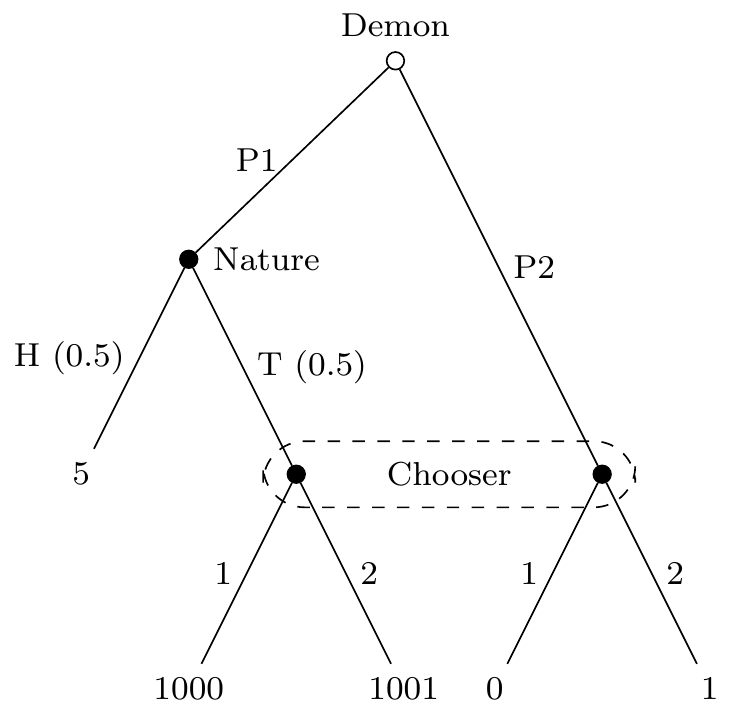
\includegraphics{four-problems-may-19-2024_files/figure-pdf/fig-demon-then-coin-1.png}

}

\caption{\label{fig-demon-then-coin}Demon-then-Coin}

\end{figure}%

\subsection{Table}

\begin{longtable}[]{@{}ccc@{}}
\caption{Demon-then-Coin}\label{tbl-demon-then-coin}\tabularnewline
\toprule\noalign{}
& P1 & P2 \\
\midrule\noalign{}
\endfirsthead
\toprule\noalign{}
& P1 & P2 \\
\midrule\noalign{}
\endhead
\bottomrule\noalign{}
\endlastfoot
1 & 502.5 & 0 \\
2 & 503 & 1 \\
\end{longtable}

If Chooser was planning on picking 1 box, they have a little evidence
against the accuracy of Demon's predictions. If in the other games they
thought the probability that Demon mispredicted was \emph{e}, in this
case they should (if they plan to choose 1 box) have a probability of
error of roughly 2\emph{e}. But if \emph{e} was small enough to start
with, and I'll assume throughout that Demon's error likelihood is
arbitrarily small, this shouldn't make a difference.

Again, I'm going to argue that the dynamic game,
Figure~\ref{fig-demon-then-coin}, and the strategic game,
Table~\ref{tbl-demon-then-coin}, should get the same solutions. Indeed,
they should get the same solutions for the same reason the previous two
pairs of decisions should get the same solutions. That reason, I'll
argue, is the Single Choice Principle.

\subsection{Single Choice Principle}\label{sec-scp-definition}

Here is what the Single Choice Principle (hereafter, SCP) says:

\begin{quote}
\textbf{Single Choice Principle (SCP)}\\
In any decision tree in which all the nodes where Chooser acts are in a
single information set, an option is choice-worthy in the dynamic form
of the game iff it is choice-worthy in the strategic form of the game.
\end{quote}

The SCP is a highly restricted version of a claim that dynamic and
static games are in some sense equivalent. The strong version of the
view says that there is some mapping from the set of rational choices in
a tree to the set of possible choices in the strategic version of that
tree. Exactly how that mapping should be understood is tricky in the
general case, but since (a) the general principle is extremely
controversial, and (b) I'm not endorsing the general principle, I won't
fuss over the details. What I will fuss over is getting clearer about
what the SCP does and doesn't say.

The SCP doesn't just say that on any run through the game, Chooser only
makes one choice. Rather, it says that Chooser only has one possible
choice to make in the game. This point might be clearer with an example.
Imagine Chooser and Demon are playing a simple kind of ultimatum game.
Demon has to propose a split of a \$3 pot; they can either propose \$2
for Demon and \$1 for Chooser, or vice versa. Chooser then has a take it
or leave it choice. If they take, each party gets the money Demon
proposes; if they leave, each party gets \$0. Assume Demon is
arbitrarily good at predicting Chooser's strategy, and that Demon
prefers more money to less\footnote{Also assume Demon will flip a coin
  if they expect each option to have equal return}. The game tree is in
Figure~\ref{fig-ultimatum}, and the strategy table is in
Table~\ref{tbl-ultimatum}.

\subsection{Tree}

\begin{figure}

\centering{

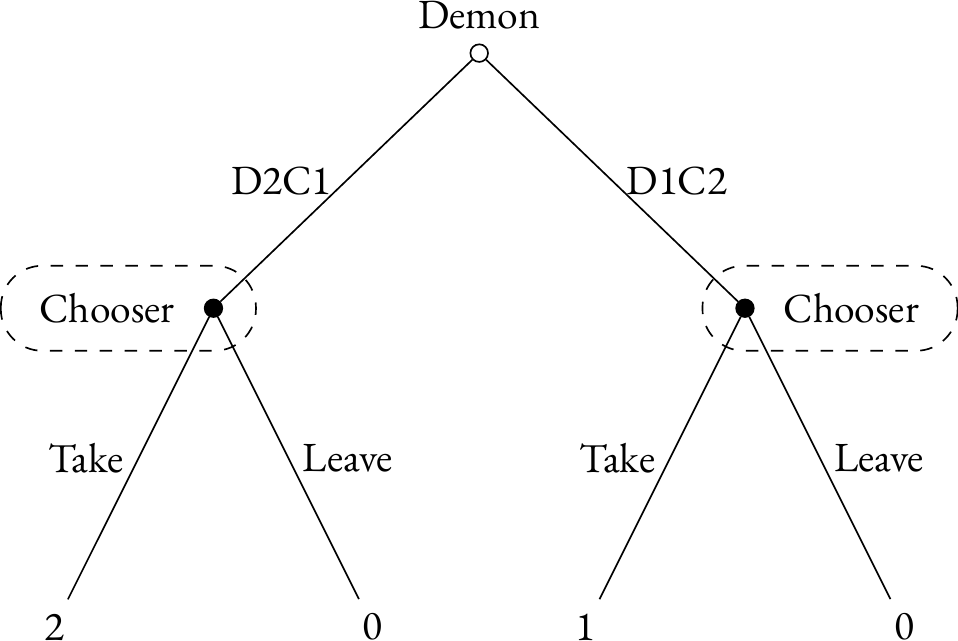
\includegraphics{four-problems-may-19-2024_files/figure-pdf/fig-ultimatum-1.png}

}

\caption{\label{fig-ultimatum}Ultimatum Game}

\end{figure}%

\subsection{Table}

\begin{table}

\caption{\label{tbl-ultimatum}Two representations of the strategic form
of ultimatum game}

\begin{minipage}[t]{0.50\linewidth}

\subcaption{\label{tbl-ultimatum-game}Demon's Decisions}

\centering{

\begin{tabular}[t]{ccc}
\toprule
 & D2C1 & D1C2\\
\midrule
\textbf{TT} & 1 & 2\\
\textbf{TL} & 1 & 0\\
\textbf{LT} & 0 & 2\\
\textbf{LL} & 0 & 0\\
\bottomrule
\end{tabular}

}

\end{minipage}%
%
\begin{minipage}[t]{0.50\linewidth}

\subcaption{\label{tbl-ultimatum-demon}Demon's Predictions}

\centering{

\begin{tabular}[t]{ccccc}
\toprule
 & PTT & PTL & PLT & PLL\\
\midrule
\textbf{TT} & 1 & 1 & 2 & 1.5\\
\textbf{TL} & 1 & 1 & 0 & 0.5\\
\textbf{LT} & 0 & 0 & 2 & 1\\
\textbf{LL} & 0 & 0 & 0 & 0\\
\bottomrule
\end{tabular}

}

\end{minipage}%

\end{table}%

Most philosophers would say that in the dynamic form of the game,
Figure~\ref{fig-ultimatum}, the only sensible thing to do is TT;
whatever the demon does, it's better to take more money than less. But
many would also say that in the strategic form,
Table~\ref{tbl-ultimatum}, some other strategy might be appropriate. For
instance, Evidential Decision Theory says that in
Table~\ref{tbl-ultimatum}, the right strategy is LT.\footnote{This is
  easier to see in Table~\ref{tbl-ultimatum-demon}; EDT says to just
  look at the numbers in the main diagonal and choose the strategy with
  the highest one.} The SCP does not rule out this combination. It will
ultimately have something to say about EDT, but it doesn't object to
this pair of views. That's because in Figure~\ref{fig-ultimatum} there
are two possible choices for Chooser to make, even if they will
ultimately only make one of them, and the SCP only applies to games with
just one possible choice. That makes it a more plausible principle, but
surprisingly does little to reduce its philosophical significance.

\section{Defending the SCP}\label{sec-scp-defence}

\subsection{A Sample Violation}\label{a-sample-violation}

The argument for the SCP is that violations of it are in various ways
incoherent. It helps to have a sample violation on the table. Imagine
Chooser is going to play the following game.

\begin{figure}

\centering{

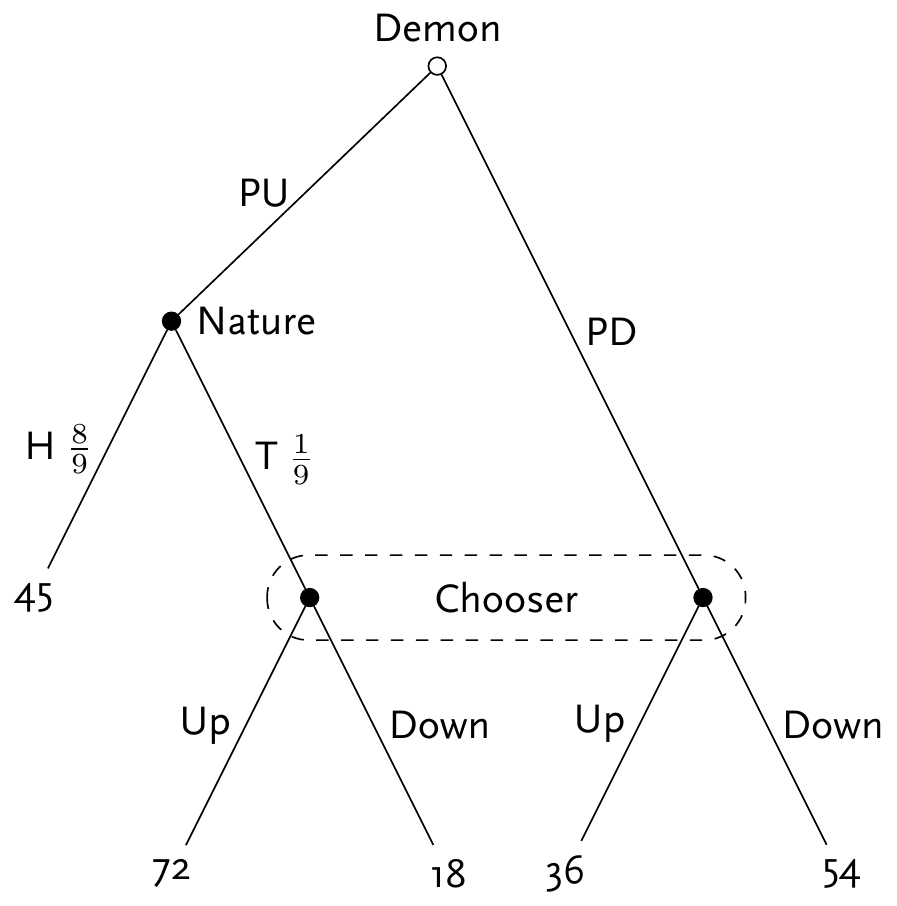
\includegraphics{four-problems-may-19-2024_files/figure-pdf/fig-sample-violation-1.png}

}

\caption{\label{fig-sample-violation}Switching Example}

\end{figure}%

Figure~\ref{fig-sample-violation} resembles
Figure~\ref{fig-demon-then-coin}, with two notable differences. First,
the coin is now weighted, and has an 8/9 chance of landing Heads.
Second, if Chooser must choose, either option is an equilibrium.

Table~\ref{tbl-sample-violation-late} shows the decision table Chooser
faces if they must make a choice in Figure~\ref{fig-sample-violation},
and \textbf{?@tbl-sample-violation-early} shows the expected payouts of
the two strategies Chooser could select.

\begin{table}

\caption{\label{tbl-sample-violation}Payout tables for
Figure~\ref{fig-sample-violation}.}

\begin{minipage}[t]{0.50\linewidth}

\subcaption{\label{tbl-sample-violation-late}Dynamic version.}

\centering{

\begin{tabular}[t]{ccc}
\toprule
 & PU & PD\\
\midrule
\textbf{Up} & 72 & 36\\
\textbf{Down} & 18 & 54\\
\bottomrule
\end{tabular}

}

\end{minipage}%
%
\begin{minipage}[t]{0.50\linewidth}

\subcaption{\label{tbl-sample-violation-late}Strategic version.}

\centering{

\begin{tabular}[t]{ccc}
\toprule
 & PU & PD\\
\midrule
\textbf{Up} & 48 & 36\\
\textbf{Down} & 42 & 54\\
\bottomrule
\end{tabular}

}

\end{minipage}%

\end{table}%

I'll take as my sample violator of the SCP a Chooser who prefers Up in
the dynamic version, and Down in the strategic version. As we'll see in
Section~\ref{sec-multiple}, many decision theorists agree with this
Chooser. But everything I say should generalise to any violation.

\subsection{Ramsey Test}\label{sec-ramsey}

To choose a strategy is to make true a bunch of conditionals. Adopting
the strategy Down in Figure~\ref{fig-sample-violation} just is saying
``If I have to choose, I'll choose Down''. As
(\citeproc{ref-RamseyTest}{\textbf{RamseyTest?}}) said, the way to tell
which such conditional to make true is to hypothetically add the
antecedent to one's stock of belief, and then decide which unconditional
claim you'd like to make true. But Chooser does not do that. If they
believed that they had to choose, they would choose Up. So their
strategic preference implies that they believe that if they had to
choose, they would choose Down, but adding the supposition that they
have to choose, they choose Up. This combination is incoherent, and so
violations of the SCP are incoherent.

I think this argument is decisive; it's incoherent to adopt a strategy
in games like Figure~\ref{fig-demon-then-coin} or
\textbf{?@fig-switching-example} that is different from what one knows
one would do if one had to carry the strategy out. That's just not how
conditionals work. But in case not everyone is convinced, I'll run
through some other arguments. The SCP will do a lot of work, and it is
worth getting the foundations as secure as possible.

\subsection{Intuitions about Change}\label{intuitions-about-change}

This argument starts with a story. Imagine the game master (GM) is
chatting to Chooser (C), before Chooser plays
\textbf{?@fig-switching-example}.

\begin{quote}
GM: What are you thinking of playing?\\
C: I might not have a choice.\\
GM: True, but assume you have to choose.\\
C: Then Up, I guess.\\
GM: You know, Demon can be really slow in making a prediction. Do you
want to write your choice down in an envelope, and we'll open it if it's
needed? C: Oh sure. I'm writing Down.\\
GM: Why did you change your mind?
\end{quote}

We could continue the conversation, but I want to focus on the
presupposition of GM's last question. It seems appropriate to presuppose
here that Chooser has changed their mind. This presupposition requires
the SCP. If the SCP is false, Chooser has simply given different answers
to different questions. First they were asked what to do in the dynamic
game, and they said Up. Then they were asked what to do in the strategic
game, and they said Down. Giving different answers to different
questions is not changing one's mind.

GM's question seems appropriate. Chooser was first asked what they
planned to do in a particular situation. Then they were asked for a
strategy that would only be activated in that very situation. When they
give different answers to those questions, it sounds like they changed
their mind. That implies the questions are fundamentally the same, which
is what the SCP says.

\subsection{Unifying the Examples}\label{sec-unity}

Philosophers do not agree about Newcomb's Problem. But they do agree
that in each of the examples in Section~\ref{sec-newcomb}, the same
choice is rational in the strategic and dynamic form of the game. This
isn't because they think that in general strategic and dynamic forms are
equivalent. Indeed, for many theorists there is no unifying story about
why each of these pairs of problems gets the same answer. It is just a
fact that the theory treats the dynamic and strategic problems the same
way.

I think it is better to have an explanation for why each of the pairs of
problems gets the same answers, and for that explanation to be the same
across the three pairs. The SCP provides such an explanation, and that's
a point in its favour.

\subsection{No Reward}\label{no-reward}

One reason that I introduced
Figure~\ref{fig-ultimatum}/Table~\ref{tbl-ultimatum} earlier is that
it's the kind of case where it's most plausible that the strategic and
dynamic choices might be distinct. Think about the pair of choices that
EDT recommends: in the dynamic game, play TT; in the strategic game,
play LT. While I ultimately disagree with this, I do think this is a
plausible thing for EDT to say. The strategy LT has two big advantages
that some will think make up for the fact that it is not what one would
do dynamically. First, it differs from the dynamically rational play
only in a situation which is, conditional on being played, highly
unlikely to come about. Second, there is a reward, at least in
expectation, for playing this dynamically irrational strategy; the
strategy has a payout of 2 while the dynamically rational strategy only
has a payout of 1. Either one of these facts will, at least to some
people, make it rational to treat dynamic and strategic games
differently; what's distinctive about
Figure~\ref{fig-ultimatum}/Table~\ref{tbl-ultimatum} is that both
reasons are there.

In dynamic problems where the SCP applies, neither of these reasons can
apply. There is no possible strategic advantage to playing the
dynamically irrational strategy. There is no parallel to saying, ``I'm
playing LT because, even though leaving money would be irrational, I
almost certainly won't have to carry that part of the strategy out, and
in exchange for this tiny risk, I'm getting rewarded.'' Doing something
dynamically irrational at the only point one can possibly move can't
have advantages elsewhere; you're going to get the same payout elsewhere
no matter what. So whatever reason one could have in other cases for
treating dynamic and strategic problems separately can't apply here;
there isn't enough of an `elsewhere' for one's bad decision at the one
and only place one moves to be compensated.

\subsection{Sure Thing}\label{sec-surething}

Finally, there is one very natural argument for the SCP that for various
reasons I don't want to lean on too heavily. If Chooser violates the
SCP, then they violate the Sure Thing Principle. They think Up is at
least as good as Down both conditional on the game ending without them
making a choice, and on that not happening. But they think Down is
better overall. If Sure Thing can be taken as a basic assumption, the
SCP immediately follows.

There are three problems with this line of reasoning. The first is
pragmatic. It's well known that various theories I'm arguing against
here, like EDT, and Buchak's non-standard treatment of risk, violate
Sure Thing. It's not a new argument against them to say that they
violate the SCP, if the only reason to believe the SCP is Sure Thing.
The second is that it isn't obvious that the theories that are best
supported by the SCP are not consistent with Sure Thing. Dmitri
(\citeproc{ref-Gallow202x}{\textbf{Gallow202x?}}) argues that what he
calls `stable' decision theories are bound to violate Sure Thing. It's
arguable that his arguments can be generalised to provide a reason to
think theories supported by the SCP (which will typically not be stable
in his sense) also violate Sure Thing. And the third is that even if
this argument fails, there is a bad company objection to Sure Thing that
I'll get to in \textbf{?@sec-negdom}. So it's useful that we have the
other four arguments to fall back on.

\section{Flagging Assumptions}\label{sec-flagging}

I'm going to make three assumptions in what follows, and it helps to
have them on the table.

One is that we can sensibly talk about demons who are arbitrarily
accurate at predicting Chooser's strategy. One reason for making this
assumption is that all the problems we discuss could be rephrased if we
just assumed Demon was at least epsilon better than chance at predicting
Chooser's strategy, and this is a realistic assumption. It would
complicate the algebra considerably in what follows to do this, without
making the examples clearer. A second reason for making the assumption
is that standard approaches to game theory assume each player is a demon
who can predict the other players' strategies with arbitrary precision,
so we're just deferring to orthodox opinion in a notable research topic
by making this assumption.

A second is that decision problems are fully specified by setting out
the states (assumed to be causally independent of actions), the
available actions, the payoffs for each state-action pair, and the
conditional probability of each state given each action. Here I'm
following (\citeproc{ref-Gallow202x}{\textbf{Gallow202x?}}), whose
formalism for decision problems only includes places for these
variables. This is a more substantive assumption. Some decision
theorists think we need to include other factors, such as Chooser's
prior unconditional probabilities for various states, or Chooser's
attitude to risk. I'll note below where this assumption matters, but in
general I'll be following Gallow in making this assumption.

And a third is that in any dynamic choice, a choice at a point is
permissible only if it would be permissible were that starting point of
a decision problem. This rules out so-called \emph{sophisticated}
approaches to dynamic choice. And I'll come back in
\textbf{?@sec-dual-mandate} to what happens if this assumption is
relaxed.

\section{Problem 1: Demons and Multiple Equilibria}\label{sec-multiple}

\textbf{?@tbl-demon-generic} is a completely generic form of a 2*2
decision problem involving demons. Without loss of generality, I'll
assume all payouts are positive. I'll also assume all payouts are
distinct; dropping this requires fussing about edge cases that are not
relevant here.\footnote{These edge cases are important for thinking
  about the significance of weak dominance, but that's not relevant to
  this paper.}

\begin{longtable}[]{@{}ccc@{}}
\caption{A generic demon
problem}\label{tbl-generic-demon}\tabularnewline
\toprule\noalign{}
& PU & PD \\
\midrule\noalign{}
\endfirsthead
\toprule\noalign{}
& PU & PD \\
\midrule\noalign{}
\endhead
\bottomrule\noalign{}
\endlastfoot
\textbf{Up} & \emph{a} & \emph{b} \\
\textbf{Down} & \emph{c} & \emph{d} \\
\end{longtable}

Say that an option is a (strict) equilibrium if, assuming Demon predicts
correctly, Chooser's payout for choosing it is (strictly) greater than
their payout for choosing any other option. The focus of this section is
only problems where both Up and Down are strict equilibria. In
particular, focus on problems that satisfy these three constraints.

\begin{enumerate}
\def\labelenumi{\arabic{enumi}.}
\tightlist
\item
  \emph{a} \textgreater{} \emph{c}, and \emph{d} \textgreater{}
  \emph{b}.
\item
  \emph{a} \textgreater{} \emph{d}.
\item
  \emph{b} \textgreater{} \emph{c}.
\end{enumerate}

The first says that Up and Down are both strict equilibria. The second
says that Up has the highest payout among the equilibria. The third says
that Up has a higher off-equilibrium payout than Down does. Many
theorists who disagree about other questions in decision theory say that
these three facts suffice to make Up uniquely choice-worthy.

Evidential Decision Theorists say that 2 alone suffices for choosing Up
over Down.

Consider next the theory that says only equilibria are choice-worthy,
and among equilibria, one should choose the equilibrium with the highest
expected payout. Versions of this theory are endorsed by Jeffrey
(\citeproc{ref-Jeffrey1983}{1983}), Arntzenius
(\citeproc{ref-Arntzenius2008}{2008}), and
(\citeproc{ref-Gustafson2011}{\textbf{Gustafson2011?}}). Given 1 and 2,
this theory says to choose up.

Finally, consider the theory that says one should (in two options games)
minimise possible regret. That is, one should choose Up if the possible
Regret from choosing Up, \emph{d}~-~\emph{b}, is less than the possible
regret from choosing Down, \emph{a}~-~\emph{c}.
(\citeproc{ref-Wedgwood201x}{\textbf{Wedgwood201x?}}), Gallow
(\citeproc{ref-Gallow2020}{2020}), Podgorski
(\citeproc{ref-Podgorski2022}{2022}), and
(\citeproc{ref-Barnett202x}{\textbf{Barnett202x?}}) endorse this claim,
though they go on to say very different things about cases with three or
more options. Given constraints 2 and 3, these theories also say to
choose Up.

I'll argue that in any such problem, both Up and Down are choice-worthy.
I'm not the first to say this. Jack
(\citeproc{ref-Spencer202x}{\textbf{Spencer202x?}}) and Melissa Fusco
(\citeproc{ref-Fuscond}{n.d.}) also say that both equilibria are
choice-worthy.\footnote{Fusco and Spencer disagree on a lot of other
  questions, and I think the SCP tends to favour Fusco's side of their
  disagreement, but it would be a huge digression to sort out those
  details.} This implies that in any problem where Up and Down are both
strict equilibria, they are both choice-worthy, since there is nothing
more that could make Up uniquely choice-worthy. Just what is the
relationship between being an equilibrium and being choice-worthy is a
question for another day, but in 2*2 games, they pick out the same
options.

Consider the dynamic game shown in Figure~\ref{fig-edt}.

\begin{figure}

\centering{

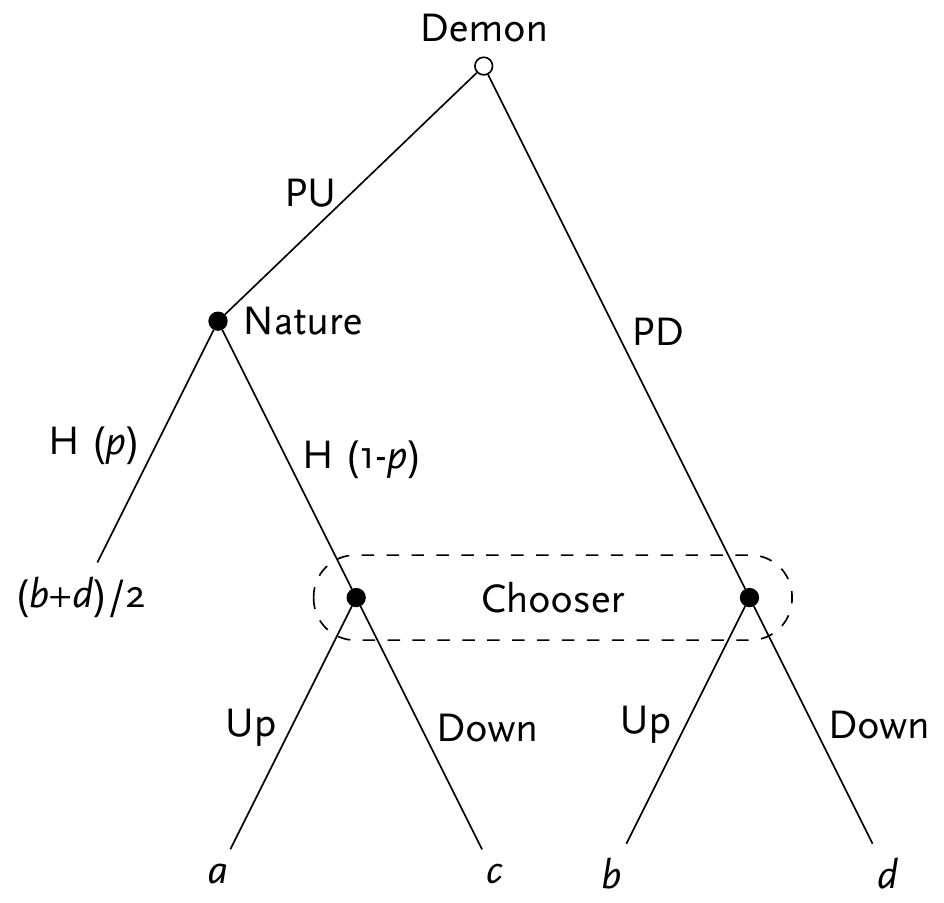
\includegraphics{four-problems-may-19-2024_files/figure-pdf/fig-edt-1.png}

}

\caption{\label{fig-edt}A tree that shows SCP is inconsistent with
several theories.}

\end{figure}%

The payouts on the right are taken from Table~\ref{tbl-generic-demon},
and the payout if the game exits without a choice is half way between
the two payouts if Demon predicts Down. I've left the probability of
exit if Demon predicts Up as a variable \emph{p}. The decision tables
for the one choice in the dynamic game, and the strategic choice for the
whole game, are in Table~\ref{tbl-edt}.

\begin{table}

\caption{\label{tbl-edt}Payout tables for Figure~\ref{fig-edt}.}

\begin{minipage}[t]{0.50\linewidth}

\subcaption{\label{tbl-edt-late}Dynamic version.}

\centering{

\begin{tabular}[t]{ccc}
\toprule
 & PU & PD\\
\midrule
\textbf{Up} & \emph{a} & \emph{b}\\
\textbf{Down} & \emph{c} & \emph{d}\\
\bottomrule
\end{tabular}

}

\end{minipage}%
%
\begin{minipage}[t]{0.50\linewidth}

\subcaption{\label{tbl-edt-late}Strategic version.}

\centering{

\begin{tabular}[t]{ccc}
\toprule
 & PU & PD\\
\midrule
\textbf{Up} & \emph{p}(\emph{b}+\emph{d})/2 +
(1-\emph{p})\emph{a} & \emph{b}\\
\textbf{Down} & \emph{p}(\emph{b}+\emph{d})/2 +
(1-\emph{p})\emph{c} & \emph{d}\\
\bottomrule
\end{tabular}

}

\end{minipage}%

\end{table}%

If \emph{p} is large enough, then in \textbf{?@tbl-edt-early}, the
bottom-right will be larger than the top-left, and the bottom-left will
be larger than the top-right. So if constraints 1-3 are sufficient
conditions for one option to be uniquely choice-worthy, then if \emph{p}
is large enough, Down will be uniquely choice-worthy in
\textbf{?@tbl-edt-early}. But Up is uniquely choice-worthy in
Table~\ref{tbl-edt-late}, so this will violate the SCP.

How large does \emph{p} have to be? As long as
\emph{p}~\textgreater~(2\emph{a}~‑~2\emph{d})/(2\emph{a}~‑~\emph{b}~‑~\emph{d}),
then the bottom-left will be greater than the top-right. This is
consistent with \emph{p}~\textless~1, since
\emph{d}~\textgreater~\emph{b}. As long as
\emph{p}~\textgreater~(2\emph{b}~‑~2\emph{c})/(\emph{b}~+~\emph{d}~‑2\emph{c}),
then the bottom-right will be greater than the top-left. Again, since
\emph{d}~\textgreater~\emph{b}, this is consistent with
\emph{p}~\textless~1. We can guarantee both conditions are met if:

\[
p = 1 - \frac{(d-b)^2}{(2a-b-d)(b+d-2c)}
\]

Assume we use the values from Table~\ref{tbl-sample-violation-late}, so
\emph{a}~=~72, \emph{b}~=~36, \emph{c}~=~18, and \emph{d}~=~54. Then
this formula says that \emph{p}~=~1/9. If we set \emph{p} to 1/9, we get
the tree shown in Figure~\ref{fig-sample-violation}. What I've argued
here is that that example is perfectly general. If constraints 1-3
suffice for Up being uniquely choice-worthy, then any game where there
are two equilibria but Up is uniquely choice-worthy can be embedded in a
dynamic game where it is the game Chooser will face if they ever have to
choose, but in the strategic form of the game, Down is uniquely
choice-worthy. So saying 1-3 suffices for Up being uniquely
choice-worthy leads to systematic violations of the SCP. Since the SCP
is true, these theories must be false.

If constraints 2 and 3 don't suffice to say that a particular strict
equilibrium in a 2\emph{2 game is not choice-worthy, it's hard to see
what further constraints could make a difference. So I conclude that, if
the SCP is true, then in 2}2 games with two strict equilibria, both
options are choice-worthy. This shows that
(\citeproc{ref-Spencer202x}{\textbf{Spencer202x?}}) and Fusco
(\citeproc{ref-Fuscond}{n.d.}) are right about these

That's a case where a theorist who thinks constraints 1-3 suffice for Up
being uniquely choice-worthy will violate the SCP. As we noted at the
start of this section, many theories do say those constraints suffice
for unique choice-worthiness, so they are all wrong.

In a 2*2 game with multiple strict equilibria, the only theory that's
compatible with the SCP, and hence the only plausible theory, is that
both equilibria are choice-worthy.

\section{Problem 2: Ordering}\label{sec-ordering}

\subsection{Introducing the Problem}\label{sec-ordering-intro}

Standard approaches to decision theory assign to Chooser a probability
function and a utility function, both defined over (some) propositions.
The domain of each function is some subset of the reals; the interval
{[}0,1{]} for the probability, and some bounded interval for the
utilities. The real numbers have a distinctive topology. Among other
things, they are totally ordered: for any two numbers, either one is
greater, or they are equal. So assuming that probabilities and utilities
are numerical involves assuming that for any two propositions, the
probability(/utility) of the first is either greater than, less than, or
equal to, that of the other. Call this assumption Ordering.

Ordering is controversial, both for probabilities and utilities. For
probabilities, it has been criticised since Keynes's \emph{Treatise on
Probability} (\citeproc{ref-Keynes1921}{1921}), and in recent times has
been criticised by, among others, Peter Walley
(\citeproc{ref-Walley1991}{1991}) and James Joyce
(\citeproc{ref-Joyce2010}{2010}). For utilities, the most prominent
contemporary critic is Ruth Chang (\citeproc{ref-Chang2002}{2002},
\citeproc{ref-Chang2015}{2015}).

Just like there are many critics of Ordering, there are many defenders.
Dorr, Nebel, and Zuehl (\citeproc{ref-DorrEtAl2023}{2023}) defend it on
semantic grounds. Adam Elga (\citeproc{ref-Elga2010}{2010}) argues that
violations of Ordering for probabilities leads to susceptibility to a
money pump. Johan Gustafsson (\citeproc{ref-Gustafsson2022}{2022}) makes
a similar in favour of Ordering for utilities.

Even critics of Ordering have noted its unintuitive characteristics.
Bradley and Steele (\citeproc{ref-BradleySteele2016}{2016}) argue that
violations of Ordering for probabilities imply it can be rational to pay
to avoid information. Harvey Lederman (\citeproc{ref-Ledermannd}{2024})
argues that violations of Ordering for utilities leads to violations of
a principle he calls Negative Dominance, which I'll return to below.

Both Bradley and Steele, and Lederman, think that ultimately Ordering
should be rejected, and we should live with these unintuitive results.
They are both pointing out troubling features of their own view.
(Something philosophers should do more often.) In each case it isn't
hard to convert the argument they give to a problem for the other kind
of Ordering violation. If Ordering fails for utilities, a Bradley and
Steele-style argument shows that it is worth paying to avoid
information, and if it fails for probabilities, a Lederman style
argument shows that Negative Dominance fails.

I'm going to offer a new defence of Ordering violations. The defence has
two parts. In this section, I'll argue that even if Ordering holds for
probabilities and for values of states, it does not hold for values of
actions. A bit loosely, even if Ordering is true for preferences over
ends, it isn't true for preferences over means. This shows we have
independent reason to reject any principle that entails Ordering is true
in general. That includes many of the premises in arguments that have
been offered against Ordering. Then in \textbf{?@sec-dual-mandate}, I'm
going to argue that many of the criticisms of views that permit Ordering
violations presuppose a false view about how rational dynamic choice
works.

\subsection{Argument from Sweeteners}\label{sec-sweeteners}

In Section~\ref{sec-multiple} I argued that in
Table~\ref{tbl-sample-violation-late}, both Up and Down are
choice-worthy. This is consistent with Ordering only if Chooser is
indifferent between Up and Down. If Chooser is indifferent, then
`sweetening' one of the options, by increasing its payout in all states,
should break the tie between them. But it doesn't. If we start with
Table~\ref{tbl-edt-late} and add 1 to the payout for Up, we get
Table~\ref{tbl-sweetened}. And the argument in
Section~\ref{sec-multiple} shows that both Up and Down are choice-worthy
in Table~\ref{tbl-sweetened}.

\begin{longtable}[]{@{}ccc@{}}
\caption{Table~\ref{tbl-sample-violation-late} with \textbf{Up}
sweetened by 1.}\label{tbl-sweetened}\tabularnewline
\toprule\noalign{}
& PU & PD \\
\midrule\noalign{}
\endfirsthead
\toprule\noalign{}
& PU & PD \\
\midrule\noalign{}
\endhead
\bottomrule\noalign{}
\endlastfoot
\textbf{Up} & 73 & 37 \\
\textbf{Down} & 18 & 54 \\
\end{longtable}

So the SCP implies that Ordering fails in cases like these. Up and Down
are both choice-worthy, so neither is better than the other, and they
aren't equally good.

\subsection{Argument from Beta}\label{sec-beta}

There is something odd about using preference orderings in an empirical
theory of choice. We never observe preference orderings; we only ever
observe choices. A tradition tracing back to
(\citeproc{ref-Samuelson1937}{\textbf{Samuelson1937?}}) says decision
theory should start with choice dispositions, not preferences. For any
set of options S, let C(S) be the set of options Chooser regards as
choice-worthy.\footnote{Empirically, Chooser may select different
  members of S on different occasions.} This need not be a radical break
with the idea that decision theory is based around preferences. Given
some intuitive constraints on C, we can generate a preference relation
out of it, and that preference relation will satisfy Ordering. It turns
out, however, that the SCP is inconsistent with some of those
constraints.

Amartya (\citeproc{ref-Sen197x}{\textbf{Sen197x?}}) noted that (given
some other intuitive but not uncontroversial constraints), Ordering is
equivalent to the following condition on C. He gave it the unmemorable
name Principle Beta.

\begin{description}
\tightlist
\item[Beta]
If S \subseteq S', and \{A, B\} \subseteq C(S), then A \in C(S') iff B
\in C(S').
\end{description}

That is, if A and B are both initially choice-worthy, then after some
options are added, either they are both choice-worthy, or neither
is.\footnote{To see why this might be plausible, imagine each option has
  a numerical value, and the choice-worthy ones are those with maximal
  value.} If Beta fails, then either Ordering fails, or something much
less intuitive than Ordering or Beta fails. And the SCP is inconsistent
with Beta.

Extend Table~\ref{tbl-sample-violation-late} so there is a third option:
eXit. This option returns 60 whatever Demon does. And if Demon predicts
eXit, they flip a fair coin to decide whether to play PU or PD. So the
table looks like Table~\ref{tbl-beta-violation}.

\begin{longtable}[]{@{}ccc@{}}
\caption{A violation of Principle
Beta}\label{tbl-beta-violation}\tabularnewline
\toprule\noalign{}
& PU & PD \\
\midrule\noalign{}
\endfirsthead
\toprule\noalign{}
& PU & PD \\
\midrule\noalign{}
\endhead
\bottomrule\noalign{}
\endlastfoot
\textbf{Up} & 73 & 37 \\
\textbf{Down} & 18 & 54 \\
\textbf{eXit} & 60 & 60 \\
\end{longtable}

In this table, Down is not choice-worthy, since it is dominated. So
although the SCP says that C(\{U,~D\})~=~(\{U,~D\}),
C(\{U,~D,~X\})~=~(\{U,~X\}), violating Beta. So the SCP is inconsistent
with Ordering.

\subsection{Argument from Dominance}\label{sec-neg-dom}

Harvey Lederman (\citeproc{ref-Ledermannd}{2024}) notes that given some
other plausible assumptions, Ordering is inconsistent with a principle
he calls Negative Dominance.\footnote{Though note that, like Sen,
  Lederman raises doubts about these `other plausible assumptions'. Note
  also that I've rephrased his principle a little to match the notation
  of this paper.}

\begin{description}
\tightlist
\item[Negative Dominance]
If \emph{p} is a lottery proposition, and A~\textgreater~B, then either
A~\textgreater{}\textsubscript{\emph{p}}~B, or
A~\textgreater\textasciitilde{}\neg *p*\textasciitilde~B.
\end{description}

In \textbf{Negative Dominance}, \textgreater{} is a strict preference
relation, and \textgreater{}\textsubscript{\emph{p}} is the preference
relation conditional on \emph{p}. The principle says that if A is
strictly preferred to B, it also must be strictly preferred conditional
on at least one outcome of a lottery. Most theories that violate
Ordering violate Negative Dominance, and conversely most theories that
violate Negative Dominance violate Ordering. Given the SCP, it seems
plausible Negative Dominance fails. Let H be that a particular fair coin
lands Heads, T that it lands Tails, H8 a bet that pays 8 if H and 0
otherwise, and T8 a bet that pays 8 if T and 0 otherwise. In
Table~\ref{tbl-negdom}, Chooser can plau Up, Down or eXit, and Demon has
made an arbitrarily accurate prediction, but since PX is not an option,
they'll flip a coin to decide between PU and PD if they predict eXit.

\begin{longtable}[]{@{}ccc@{}}
\caption{A violation of Negative
Dominance}\label{tbl-negdom}\tabularnewline
\toprule\noalign{}
& PU & PD \\
\midrule\noalign{}
\endfirsthead
\toprule\noalign{}
& PU & PD \\
\midrule\noalign{}
\endhead
\bottomrule\noalign{}
\endlastfoot
\textbf{Up} & 1+H8 & 0 \\
\textbf{Down} & 0 & 1+T8 \\
\textbf{eXit} & 2 & 2 \\
\end{longtable}

This is a violation of Negative Dominance given these three assumptions.

\begin{enumerate}
\def\labelenumi{\arabic{enumi}.}
\tightlist
\item
  A strategy is not choice-worthy if it is dominated, including if it is
  dominated by a mixed strategy.
\item
  If A is choice-worthy and B is not, then A~\textgreater~B.
\item
  If B is choice-worthy and A is available, then ¬(A~\textgreater~B).
\end{enumerate}

In Table~\ref{tbl-negdom}, eXit is dominated by a 50/50 mix of Up and
Down, so it is not choice-worthy. But conditional on either way the coin
lands, it is choice-worthy. Conditional on Heads, Table~\ref{tbl-negdom}
becomes Table~\ref{tbl-negdom-heads}.

\begin{longtable}[]{@{}ccc@{}}
\caption{Table~\ref{tbl-negdom} conditional on
Heads}\label{tbl-negdom-heads}\tabularnewline
\toprule\noalign{}
& PU & PD \\
\midrule\noalign{}
\endfirsthead
\toprule\noalign{}
& PU & PD \\
\midrule\noalign{}
\endhead
\bottomrule\noalign{}
\endlastfoot
\textbf{Up} & 9 & 0 \\
\textbf{Down} & 0 & 1 \\
\textbf{eXit} & 2 & 2 \\
\end{longtable}

In Table~\ref{tbl-negdom-heads}, Down is dominated and so eliminated.
And post-deletion, the arguments in Section~\ref{sec-multiple} show both
options are choice-worthy. A similar argument shows that eXit is
choice-worthy conditional on Tails. So given the three assumptions,
which seem fairly plausible links between choice-worthiness and
preference, the SCP implies that Negative Dominance fails.

Most theories which reject Ordering also violate a principle I'll call
\textbf{Strict Dominance}. This is roughly a converse to Lederman's
Negative Dominance.

\begin{description}
\tightlist
\item[Strict Dominance]
If \emph{p} is a lottery proposition, and
A~\textgreater{}\textsubscript{\emph{p}}~B and
A~\textgreater\textasciitilde{}\neg *p*\textasciitilde~B. then
A~\textgreater~B.
\end{description}

Strict Dominance isn't quite the traditional Sure Thing Principle, since
it uses strict preference and the Sure Thing Principle normally uses at
least as good as. But it's fairly close. Close enough, indeed, that it's
a bit disconcerting it fails. This is why I mentioned back in
Section~\ref{sec-surething} that there is a bad company objection to the
Sure Thing principle.

\section{The Four Problems}\label{the-four-problems}

When a student starts decision theory, they are introduced to a view
that is simple, elegant, and wrong. The view starts by assuming that
Chooser, has some actions \emph{A} available, with \emph{a} an arbitrary
action from \emph{A}. There are some possible states \emph{S}, with
\emph{s} an arbitrary such state. Two numerical functions are given: a
probability function Pr over states, and a value function \emph{V} over
pairs of actions and states.

The simple, elegant, and wrong theory is that Chooser should value each
act \emph{a} by its expected value, and choose the one with the highest
value. That is, Chooser should select \emph{a} to maximise
Σ\textsubscript{\emph{s}~∈~\emph{S}}~Pr(\emph{s})\emph{V}(\emph{as}).

If Chooser has any causal influence over the states, this theory gives
bad advice. Assume \emph{A} is \{\emph{a}, \emph{b}\}, \emph{S} is
\{\emph{s},~\emph{t}\}, and \emph{a} will cause \emph{s} to be actual,
while \emph{b} will cause \emph{t}. And assume \emph{V} is described in
Table~\ref{tbl-joycewindow}.

\begin{longtable}[]{@{}ccc@{}}
\caption{A counterexample to the simple
theory.}\label{tbl-joycewindow}\tabularnewline
\toprule\noalign{}
& \emph{s} & \emph{t} \\
\midrule\noalign{}
\endfirsthead
\toprule\noalign{}
& \emph{s} & \emph{t} \\
\midrule\noalign{}
\endhead
\bottomrule\noalign{}
\endlastfoot
\emph{a} & 1 & 1001 \\
\emph{b} & 0 & 1000 \\
\end{longtable}

In Table~\ref{tbl-joycewindow} Chooser should do \emph{b} and bring
about the best state, but whatever Pr says, the simple theory says to do
\emph{a}. So far every decision theorist would agree. But here agreement
ends. There is no agreement on either why the simple theory fails in
this case, or what should go in its place.

Evidential decision theorists such as Arif Ahmed
(\citeproc{ref-Ahmed2014}{2014}) say Chooser should value options using
this formula.

\begin{description}
\tightlist
\item[EDT]
\emph{V}(\emph{a}) = Σ\textsubscript{\emph{s}~∈~\emph{S}}~Pr(\emph{s}
\textbar{} \emph{a})\emph{V}(\emph{as})
\end{description}

EDT modifies the simple theory by replacing an unconditional probability
with a conditional probability. This leads to striking results in a
version of Table~\ref{tbl-joycewindow} where the states are causally
independent of the actions, but evidentially connected. Following Nozick
(\citeproc{ref-Nozick1969}{1969}), imagine that Demon has predicted
Chooser's choice. There is no backwards causation, so Chooser's choice
is causally independent of Demon's prediction. But Chooser believes
Demon is incredibly reliable, so Pr(\emph{s}~\textbar~\emph{a})~≈~1, and
Pr(\emph{t}~\textbar~\emph{b})~≈~1. We'll represent this setup in
Table~\ref{tbl-newcomb}. In general, when the states are predictions of
Demon, I'll label it as \textbf{PX}, meaning X is Predicted.

\begin{longtable}[]{@{}ccc@{}}
\caption{Newcomb's Problem}\label{tbl-newcomb}\tabularnewline
\toprule\noalign{}
& \textbf{PU} & \textbf{PD} \\
\midrule\noalign{}
\endfirsthead
\toprule\noalign{}
& \textbf{PU} & \textbf{PD} \\
\midrule\noalign{}
\endhead
\bottomrule\noalign{}
\endlastfoot
\textbf{U} & 1 & 1001 \\
\textbf{D} & 0 & 1000 \\
\end{longtable}

In Table~\ref{tbl-newcomb}, EDT says that Chooser should do \emph{a}.
Many philosophers rejected this because Chooser is better off whatever
Demon has done. One theory that captures that intuition uses CfDT as the
formula for valuing actions.\footnote{The canonical statement of this
  view is Gibbard and Harper (\citeproc{ref-GibbardHarper1978}{1978}).
  Recently Brian Hedden (\citeproc{ref-Hedden2023}{2023}) has argued
  that this theory is preferable to \emph{Causal} Decision Theory,
  properly so called. I'm sympathetic to the reply offered by Dmitri
  Gallow (\citeproc{ref-Gallowndppq}{n.d.}) that CfDT just is what
  Causal Decision Theorists in the 1970s and 1980s were typically
  defending.}

\begin{description}
\tightlist
\item[CfDT]
\emph{V}(\emph{a}) = Σ\textsubscript{\emph{s}~∈~\emph{S}}~Pr(\emph{a} □→
\emph{s})\emph{V}(\emph{as})
\end{description}

Sometimes this is called \textbf{Causal} Decision Theory, but I won't
use that name; some causal theories use very different value functions.
I'll use ``Causal Decision Theory'' to name a family of theories, and
CfDT will be a distinctive member of that family.

Another theory in that family says that the simple theory was
essentially correct, it was just applied at the wrong time. This theory,
hereafter Gamified Decision Theory (GDT), is based on two claims. First,
the relevant probabilities over states are those Chooser has at the end
of deliberation, not the start. Second, when using those \emph{ex post}
probabilities, the simple theory is fine. In symbols, the core formula
that GDT uses is this, where Pr′ is the probability over states at the
end of deliberation.

\begin{description}
\tightlist
\item[GDT]
V(a) =
Σ\textsubscript{\emph{s}~∈~\emph{S}}~Pr′(\emph{s})\emph{V}(\emph{as})
\end{description}

GDT says that only options that have maximal value using this formula
are choice-worthy.\footnote{My preferred version of GDT adds several
  more constraints to this, e.g., to rule out weakly dominated options
  and to get the right verdict in the beer-quiche game (Cho and Kreps
  (\citeproc{ref-ChoKreps1987}{1987})), but this paper will focus on
  cases where maximising this formula is necessary and sufficient for
  choice-worthiness.} This allows that different options, with different
values, could be choice-worthy. All that matters is that given the
probability distribution over states that Chooser has when they have
decided to perform an act, that act is utility maximising. In
Table~\ref{tbl-first-coord}, GDT says that both Up and Down are
choice-worthy.

\begin{longtable}[]{@{}ccc@{}}
\caption{An asymmetric coordination
problem}\label{tbl-first-coord}\tabularnewline
\toprule\noalign{}
& \textbf{PU} & \textbf{PD} \\
\midrule\noalign{}
\endfirsthead
\toprule\noalign{}
& \textbf{PU} & \textbf{PD} \\
\midrule\noalign{}
\endhead
\bottomrule\noalign{}
\endlastfoot
\textbf{U} & 3 & 0 \\
\textbf{D} & 0 & 2 \\
\end{longtable}

One of our four problems is to work out which of these theories is
right. I'll be arguing for GDT.

\subsection{Non-Linearity}\label{sec-intro-ordering}

Standard approaches to decision theory assign to Chooser a probability
function and a utility function, both defined over (some) propositions.
The domain of each function is some subset of the reals; the interval
{[}0,1{]} for the probability, and some bounded interval for the
utilities. The real numbers have a distinctive topology. Among other
things, they are totally ordered: for any two numbers, either one is
greater, or they are equal. So assuming that probabilities and utilities
are numerical involves assuming, among other things, that they are also
totally ordered. That is, for any two propositions, the
probability(/utility) of the first is either greater than, less than, or
equal to, that of the other. Call this assumption Ordering.

Ordering is controversial, both for probabilities and utilities. For
probabilities, it has been criticised since Keynes's \emph{Treatise on
Probability} (\citeproc{ref-Keynes1921}{1921}), and in recent times has
been criticised by, among others, Peter Walley
(\citeproc{ref-Walley1991}{1991}) and James Joyce
(\citeproc{ref-Joyce2010}{2010}). For utilities, the most prominent
contemporary critic is Ruth Chang (\citeproc{ref-Chang2002}{2002},
\citeproc{ref-Chang2015}{2015}).

Just like there are many critics of Ordering, there are many defenders.
Dorr, Nebel, and Zuehl (\citeproc{ref-DorrEtAl2023}{2023}) defend it on
semantic grounds. Adam Elga (\citeproc{ref-Elga2010}{2010}) argues that
violations of Ordering for probabilities leads to susceptibility to a
money pump. Johan Gustafsson (\citeproc{ref-Gustafsson2022}{2022}) makes
a similar in favour of Ordering for utilities.

Even critics of Ordering have noted its unintuitive characteristics.
Bradley and Steele (\citeproc{ref-BradleySteele2016}{2016}) argue that
violations of Ordering for probabilities leads to thinking it is
acceptable to pay to avoid information.\footnote{It's uncontroversial
  that in some cases we pay to avoid information, e.g., we take efforts
  to avoid spoilers for movies. Even if the information doesn't change
  the value of the final product, we might pay to avoid it if the
  information is not partitional (\citeproc{ref-Das2023}{Das 2023}), or
  we don't know we'll conditionalise (\citeproc{ref-Nethnd}{Neth,
  n.d.}). But if none of these three conditions are met, and
  probabilities and utilities satisfy Ordering, we should never pay to
  avoid information (\citeproc{ref-Blackwell1951}{Blackwell 1951}).}
Harvey Lederman (\citeproc{ref-Ledermannd}{2024}) argues that violations
of Ordering for utilities leads to violations of a principle he calls
Negative Dominance, which I'll discuss more in \textbf{?@sec-negdom}.

Both Bradley and Steele, and Lederman, think that ultimately Ordering
should be rejected, and we should live with these unintuitive results.
They are both pointing out troubling features of their own view.
(Something philosophers should do more often.) In each case it isn't
hard to convert the argument they give to a problem for the other kind
of Ordering violation. If Ordering fails for utilities, a Bradley and
Steele-style argument shows that it is worth paying to avoid
information, and if it fails for probabilities, a Lederman style
argument shows that Negative Dominance fails.

I'm going to offer a new defence of Ordering violations. The defence has
two parts. First, I'll argue that even if Ordering holds for
probabilities and for values of states, it does not hold for values of
actions. A bit loosely, even if Ordering is true for preferences over
ends, it isn't true for preferences over means. This shows we have
independent reason to reject any principle that entails Ordering is true
in general. That includes Negative Dominance\footnote{Negative Dominance
  doesn't on its own entail Ordering, but it does in conjunction with
  some other principles that I accept, and indeed will be indirectly
  defending in this paper.}, and the semantic principles Dorr et al
endorse. Second, I'm going to argue that many of the criticisms of views
that permit Ordering violations presuppose a false view about how
rational dynamic choice works. This is how I'll respond to Elga,
Gustafsson, and Bradley and Steele.

\subsection{Dynamic Choice}\label{sec-dynamic-choice}

On that note, it's time to introduce the last of our four problems -
what the general theory of rational dynamic choice should look like.
First, I'll set up how I'm conceiving of dynamic choice situations.

For the purposes of this paper, a \textbf{decision tree} is a sextuple
⟨\emph{W}, \emph{R}, \emph{V}, \emph{a}, \emph{I}, Pr⟩ such that:

\begin{itemize}
\tightlist
\item
  \emph{W} is a finite set of nodes. One of these nodes, call it
  \emph{o} for origin, is designated as the initial node.
\item
  \emph{R} is a relation on \emph{W} such that for any
  \emph{x}~∈~\emph{W}, ¬\emph{xRo}, and if \emph{y}~≠~\emph{o}, there is
  a unique \emph{x} such that \emph{xRy}. Intuitively, the decision
  problem starts at \emph{o}; proceeds in steps; can move from \emph{x}
  to \emph{y} iff \emph{xRy}; and ends when it reaches a node \emph{y}
  such that ¬∃\emph{z}: \emph{yRz}. Say that \emph{x} is a predecessor
  of \emph{y} if \emph{xR+y}, where \emph{R+} is the ancestral of
  \emph{R}.
\item
  \emph{V} is a value function, mapping terminal nodes to real numbers.
\item
  \emph{a} is a function from non-terminal nodes in \emph{W} to the set
  \{C,~D,~N\} that says who the agent is for each node. Intuitively, C
  is for Chooser, D is for Demon, and N is for Nature. That agent
  `chooses' where the game goes next.
\item
  \emph{I} is a partition of the nodes the non-terminal nodes
  \emph{x:~a(x)~=}C. The elements of this partition are called
  information sets. Intuitively, when Chooser reaches a node where they
  must choose, they know that they are in one member of this partition,
  i.e., one information set, and nothing more. Any two nodes in the same
  information set have the same number of outbound links.
\item
  Pr is a conditional probability function. It says that given a
  \emph{strategy} for Chooser, and that a particular non-terminal node
  \emph{x} which is assigned to Demon or Nature has reached, what the
  probability is that we'll move to some further node \emph{y} such that
  \emph{xRy}. If \emph{x} is assigned to Nature, this probability is
  independent of Chooser's strategy.
\end{itemize}

A \textbf{strategy} for one of the three players, Demon, Chooser or
Nature, is a function from all the nodes in the tree which are assigned
to them, to the move they will make if that node is reached.\footnote{It
  doesn't matter much for our purposes, but note that in general a
  strategy includes what to do if one reaches a node that is ruled out
  by one's own prior choices.} Given any decision tree, one can generate
a \textbf{strategic decision problem} where the possible actions are
strategies for Chooser, and the states are pairs of strategies for Demon
and strategies for Nature. One question that will be central

There are two standard positions in philosophy for how to navigate
decision trees. The \textbf{resolute} view says that Chooser should use
the correct static theory of choice to pick a strategy at the start, and
then resolutely stick with it. The \textbf{sophisticated} theory says
that Chooser should take each node as a new choice, treat their past
choices as fixed, and treat their future choices as another more-or-less
knowable part of the world, and do whatever is best given those
constraints. My view is that both of these are wrong.

The \textbf{dual mandate} approach, which I favour, says that Chooser
should adopt a strategy that makes sense and stick to it, just like the
resolute theory says, \emph{and} Chooser should make choices that make
sense at each point, just like the sophisticated theory says. It
disagrees with the two existing theories on two counts. First, it denies
that either provides a sufficient theory for a sequence of choices being
rational. Second, it says that if Chooser adopts a plan that makes sense
now, and will continue to make sense at each node conditional on
reaching that node, Chooser does not have to regard the future as
unknowable. Rather, Chooser can know that they will keep following the
sensible plan they have adopted. The point is not just that Chooser
knows they will continue to be rational. If Chooser has many rational
choices, once they adopt one, Chooser can know they'll stick to it.

I'll defend this more in \textbf{?@sec-dualmandate}, and argue that many
arguments for Ordering fail because they presuppose the Dual Mandate
theory is false.

\section{Ratificationism}\label{sec-ratify}

Go over the 4,3,2 game

Show that CDT, EDT, and most other views violate SCP

\section{Incomplete Preferences}\label{incomplete-preferences}

Again, the 4,3,2 shows this really quickly, I think this is already
written

\section{Dynamic Choice}\label{dynamic-choice}

This takes much more time.

\section{Problem 4: Risk-Sensitivity}\label{sec-buchak}

Think about what value of \emph{x} would make Chooser indifferent
between these two options, and why that would be the right value:

\begin{enumerate}
\def\labelenumi{\arabic{enumi}.}
\tightlist
\item
  \$1,000,000
\item
  A gamble that returns \$2,000,000 with probability \emph{x}, and \$0
  with probability 1-\emph{x}.
\end{enumerate}

What factors are relevant to solving for \emph{x}? One factor is the
declining marginal utility of money. Money primarily has exchange value,
and if Chooser won \$2,000,000, Chooser would exchange the second
million for things they chose not to exchange the first million for, so
the second million has less value. That's one reason that \emph{x} is
well above ½.

But is it the only reason? The orthodox answer is that it is. Lara
Buchak (\citeproc{ref-BuchakRisk}{2013}) has argued that it is not. We
also need to know how much Chooser values, or more likely disvalues,
risk. That is, we need to know how risk-seeking, or risk-averse, Chooser
is.

The orthodox view is that all we need to know are three numbers. In what
follows, let \emph{b} be Chooser's current wealth in millions, and V the
function from wealth (in millions), to utility. Since V is only
determined up to positive affine transformations, we can stipulate two
of these values for V.

\begin{itemize}
\tightlist
\item
  V(\emph{b}), stipulated to be 0.
\item
  V(\emph{b} + 1), stipulated to be 1.
\item
  V(\emph{b} + 1), which we'll label \emph{c}.
\end{itemize}

On the standard view, the gamble's value is \emph{cx}, so Chooser is
indifferent between it and the money iff \emph{x}~=~1/\emph{c}. On
Buchak's view, rational Chooser has a risk function \emph{f}, that
measures their sensitivity to risk. The function must be monotonic
increasing, with \emph{f}(0)~=~0, and \emph{f}(1)~=~1. If Chooser is
risk-averse, then typically \emph{f}(\emph{x})~\textless~\emph{x}.
Buchak's view reduces to the orthodox view if
\emph{f}(\emph{x})~=~\emph{x}. I'm going to argue that given the SCP,
\emph{f}(\emph{x}) does equal \emph{x}. I'm far from the first to argue
for \emph{f}(\emph{x})~=~\emph{x}.\footnote{See Briggs
  (\citeproc{ref-Briggs2015}{2015}) and Thoma
  (\citeproc{ref-Thoma2019}{2019}) for different arguments to the same
  conclusion.} The value of the argument here is that it uses the same
principle, the SCP, that is relevant to so many other problems.

The core of Buchak's theory is a non-standard way of valuing a gamble.
For simplicity, we'll focus on gambles with finitely many outcomes.
Associate a gamble with a random variable \emph{O}, which takes values
\emph{o}\textsubscript{1}, \ldots, \emph{o\textsubscript{n}}, where
\emph{o\textsubscript{j}}~\textgreater~\emph{o\textsubscript{i}} iff
\emph{j}~\textgreater~\emph{i}. Buchak says that the risk-weighted
expected utility of \emph{O} is given by this formula, where \emph{f} is
the agent's risk-weighting function.

\[
REU(O) = o_1 + \sum_{i = 2}^n f(\Pr(O \geq o_i))(o_i - o_{i-1})
\]

The decision rule then is simple: choose the gamble with the highest
REU.

The key notion here is the risk function \emph{f}, which we introduced
earlier. I'm going to show that if
\emph{f}(\emph{x})~=~\emph{x}\textsuperscript{2}, then we get a
violation of the SCP. This is If \emph{f} is the identity function, then
this definition becomes a slightly non-standard way of defining expected
utility. Buchak allows it to be much more general. The key constraints
are that \emph{f} is monotonically increasing, that \emph{f}(0)~=~0 and
\emph{f}(1)~=~1. In general, if \emph{f}(\emph{x})~\textless~\emph{x},
Chooser is more risk-averse than an expected utility maximiser, while if
\emph{f}(\emph{x})~\textgreater~\emph{x}, Chooser is more risk-seeking.
The former case is more relevant to everyday intuitions, and it's what
I'll focus on. Indeed, I'll focus on the case where
\emph{r}(\emph{x})~=~\emph{x}\textsuperscript{2}, which is also a case
Buchak uses a lot.

There are a number of good reasons to like Buchak's theory, but it is
inconsistent with the Single Choice Principle. I'll show this for the
case \emph{r}(\emph{x})~=~\emph{x}\textsuperscript{2}, but it's not much
harder to produce similar examples for any value of \emph{r} other than
\emph{r}(\emph{x})~=~\emph{x}. In Figure~\ref{fig-buchak} at stage 1 a
fair die will be rolled. If it lands 1 or 2, Nature moves Left; if it
lands 3 or 4, Nature moves Middle; otherwise, Nature moves Right. If
Nature moves Left, the game ends, and Chooser gets 1. Otherwise Chooser
is told that Nature did not move Left, but not whether they moved Middle
or Right. If Chooser selects Down, they get 1. If Chooser selects Up,
they get 5 if Nature moved Middle, and 0 otherwise.

\begin{figure}

\centering{

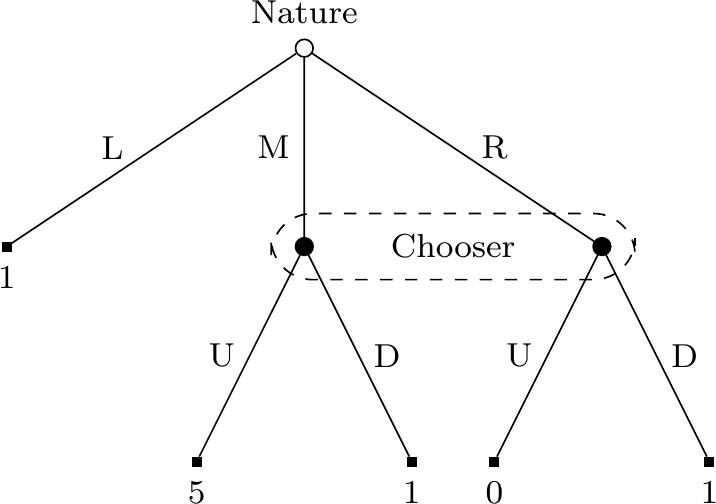
\includegraphics{four-problems-may-19-2024_files/figure-pdf/fig-buchak-1.png}

}

\caption{\label{fig-buchak}Tree Diagram of the counterexample to REU.}

\end{figure}%

Table~\ref{tbl-buchak-early} shows the strategic table of
Figure~\ref{fig-buchak}, and Table~\ref{tbl-buchak-late} shows the
decision table Chooser faces at the time they have to choose.

\begin{table}

\caption{\label{tbl-panel}Two strategy tables for
Figure~\ref{fig-buchak}.}

\begin{minipage}[t]{0.50\linewidth}

\subcaption{\label{tbl-buchak-early}The strategy table at game start.}

\centering{

\begin{tabular}[t]{cccc}
\toprule
 & \textbf{Left} & \textbf{Middle} & \textbf{Right}\\
\midrule
\textbf{Up} & 1 & 5 & 0\\
\textbf{Down} & 1 & 1 & 1\\
\bottomrule
\end{tabular}

}

\end{minipage}%
%
\begin{minipage}[t]{0.50\linewidth}

\subcaption{\label{tbl-buchak-late}The strategy table at choice time.}

\centering{

\begin{tabular}[t]{ccc}
\toprule
 & \textbf{Middle} & \textbf{Right}\\
\midrule
\textbf{Up} & 5 & 0\\
\textbf{Down} & 1 & 1\\
\bottomrule
\end{tabular}

}

\end{minipage}%

\end{table}%

In Table~\ref{tbl-buchak-early}, the REU of Down is 1 (since that's the
only possible outcome), and the REU of Up is 8/9. There is a 2/3 chance
of getting at least 1, so that's worth 4/9, and there's a 1/3 chance of
getting another 4, so that's also worth 4/9, and adding those gives 8/9.
So the optimal strategy, according to REU theory, is Down. That is, REU
says to prefer the strategy \emph{Choose Down if you have to choose} to
the strategy \emph{Choose Up if you have to choose}. But if we get to
the choice point, we're at Table~\ref{tbl-buchak-late}. And in that
table the REU of Up is 5 times 1/4, i.e., 5/4. So at that point, REU
says to choose Up. What REU says to do if you have to choose is
different to which strategy it chooses for the one and only point you
have to choose at. That is, Buchak's theory violates the SCP, and so
should be rejected.

This is far from the first objection to Buchak's view, but something
interesting follows from the connection, via the SCP, to demonic
problems. Many decision theorists reject Buchak's view about non-demonic
problems in favour of orthodox expected utility theory, but also endorse
views inconsistent with the SCP.\footnote{Evidential Decision Theorists
  reject both Buchak's view and the SCP, and in this respect they are
  far from alone.} Those theorists can't coherently use this argument
against Buchak's view. Nor can they use any other argument whose
premises entail the SCP, such as an argument from the Sure Thing
Principle. It would take too long to argue for this here, but I suspect
there is no way to do this.\footnote{Note that if we don't want to argue
  from first principles, but instead try to capture intuitions about
  cases, we should prefer Buchak's theory because of how it handles the
  Allais (\citeproc{ref-Allais1953}{1953}) paradox.} If we reject the
SCP, the weight of reasons favours Buchak's view over orthodoxy. I'll
leave this as a challenge for theorists unconvinced by
Section~\ref{sec-ratify}: what is the best argument against Buchak's
view, and in favour of expectectationist orthodoxy, whose premises do
not entail the SCP? The separation in the literature between demonic and
non-demonic problems has obscured how hard a challenge this is.

\section{Conclusion}\label{conclusion}

Paragraph about how this connects to game theory

Summary of what we've shown.

\phantomsection\label{refs}
\begin{CSLReferences}{1}{0}
\bibitem[\citeproctext]{ref-Ahmed2014}
Ahmed, Arif. 2014. \emph{Evidence, Decision and Causality}. Cambridge:
{C}ambridge {U}niversity {P}ress.

\bibitem[\citeproctext]{ref-Allais1953}
Allais, M. 1953. {``Le Comportement de l'homme Rationnel Devant Le
Risque: Critique Des Postulats Et Axiomes de l'ecole Americaine.''}
\emph{Econometrica} 21 (4): 503--46. doi:
\href{https://doi.org/10.2307/1907921}{10.2307/1907921}.

\bibitem[\citeproctext]{ref-Arntzenius2008}
Arntzenius, Frank. 2008. {``No Regrets; or, Edith Piaf Revamps Decision
Theory.''} \emph{Erkenntnis} 68 (2): 277--97. doi:
\href{https://doi.org/10.1007/s10670-007-9084-8}{10.1007/s10670-007-9084-8}.

\bibitem[\citeproctext]{ref-Blackwell1951}
Blackwell, David. 1951. {``Comparison of Experiments.''}
\emph{Proceedings of the Berkeley Symposium on Mathematical Statistics
and Probability} 2 (1): 93--102.

\bibitem[\citeproctext]{ref-BradleySteele2016}
Bradley, Seamus, and Katie Steele. 2016. {``Can Free Evidence Be Bad?
Value of Informationfor the Imprecise Probabilist.''} \emph{Philosophy
of Science} 83 (1): 1--28. doi:
\href{https://doi.org/10.1086/684184}{10.1086/684184}.

\bibitem[\citeproctext]{ref-Briggs2015}
Briggs, Ray. 2015. {``Costs of Abandoning the Sure-Thing Principle.''}
\emph{Canadian Journal of Philosophy} 45 (5): 827--40. doi:
\href{https://doi.org/10.1080/00455091.2015.1122387}{10.1080/00455091.2015.1122387}.

\bibitem[\citeproctext]{ref-BuchakRisk}
Buchak, Lara. 2013. \emph{Risk and Rationality}. Oxford: Oxford
University Press.

\bibitem[\citeproctext]{ref-Chang2002}
Chang, Ruth. 2002. {``The Possibility of Parity.''} \emph{Ethics} 112
(4): 659--88. doi:
\href{https://doi.org/10.1086/339673}{10.1086/339673}.

\bibitem[\citeproctext]{ref-Chang2015}
---------. 2015. {``Value Incomparability and Incommensurability.''} In
\emph{The Oxford Handbook of Value Theory}, edited by Iwao Hirose and
Jonas Olson, 205--24. Oxford: Oxford University Press. doi:
\href{https://doi.org/10.1093/oxfordhb/9780199959303.013.0012}{10.1093/oxfordhb/9780199959303.013.0012}.

\bibitem[\citeproctext]{ref-ChoKreps1987}
Cho, In-Koo, and David M. Kreps. 1987. {``Signalling Games and Stable
Equilibria.''} \emph{The Quarterly Journal of Economics} 102 (2):
179--221. doi: \href{https://doi.org/10.2307/1885060}{10.2307/1885060}.

\bibitem[\citeproctext]{ref-Das2023}
Das, Nilanjan. 2023. {``The Value of Biased Information.''}
\emph{British Journal for the Philosophy of Science} 74 (1): 25--55.
doi: \href{https://doi.org/10.1093/bjps/axaa003}{10.1093/bjps/axaa003}.

\bibitem[\citeproctext]{ref-DorrEtAl2023}
Dorr, Cian, Jacob M. Nebel, and Jake Zuehl. 2023. {``The Case for
Comparability.''} \emph{Noûs} 57 (2): 414--53. doi:
\href{https://doi.org/10.1111/nous.12407}{10.1111/nous.12407}.

\bibitem[\citeproctext]{ref-Elga2010}
Elga, Adam. 2010. {``Subjective Probabilities Should Be Sharp.''}
\emph{Philosophers' Imprint} 10: 1--11.

\bibitem[\citeproctext]{ref-Fuscond}
Fusco, Melissa. n.d. {``Absolution of a Causal Decision Theorist.''}
\emph{No{û}s}. doi:
\href{https://doi.org/10.1111/nous.12459}{10.1111/nous.12459}. Early
view.

\bibitem[\citeproctext]{ref-Gallow2020}
Gallow, J. Dmitri. 2020. {``The Causal Decision Theorist's Guide to
Managing the News.''} \emph{The Journal of Philosophy} 117 (3): 117--49.
doi:
\href{https://doi.org/10.5840/jphil202011739}{10.5840/jphil202011739}.

\bibitem[\citeproctext]{ref-Gallowndppq}
---------. n.d. {``Counterfactual Decision Theory Is Causal Decision
Theory.''} Pacific Philosophical Quarterly. doi:
\href{https://doi.org/10.1111/papq.12451}{10.1111/papq.12451}.

\bibitem[\citeproctext]{ref-GibbardHarper1978}
Gibbard, Allan, and William Harper. 1978. {``Counterfactuals and Two
Kinds of Expected Utility.''} In \emph{Foundations and Applications of
Decision Theory}, edited by C. A. Hooker, J. J. Leach, and E. F.
McClennen, 125--62. Dordrecht: Reidel.

\bibitem[\citeproctext]{ref-Gustafsson2022}
Gustafsson, Johan E. 2022. \emph{Money-Pump Arguments}. Cambridge:
Cambridge University Press.

\bibitem[\citeproctext]{ref-Hedden2023}
Hedden, Brian. 2023. {``Counterfactual Decision Theory.''} \emph{Mind2}
132 (527): 730--61. doi:
\href{https://doi.org/10.1093/mind/fzac060}{10.1093/mind/fzac060}.

\bibitem[\citeproctext]{ref-Humberstone2016}
Humberstone, Lloyd. 2016. \emph{Philsophical Applications of Modal
Logic}. Milton Keynes: College Publications.

\bibitem[\citeproctext]{ref-Jeffrey1983}
Jeffrey, Richard. 1983. {``Bayesianism with a Human Face.''} In
\emph{Testing Scientific Theories}, edited by J. Earman (ed.).
Minneapolis: University of Minnesota Press.

\bibitem[\citeproctext]{ref-Joyce2010}
Joyce, James M. 2010. {``A Defence of Imprecise Credences in Inference
and Decision Making.''} \emph{Philosophical Perspectives} 24 (1):
281--323. doi:
\href{https://doi.org/10.1111/j.1520-8583.2010.00194.x}{10.1111/j.1520-8583.2010.00194.x}.

\bibitem[\citeproctext]{ref-Keynes1921}
Keynes, John Maynard. 1921. \emph{Treatise on Probability}. London:
Macmillan.

\bibitem[\citeproctext]{ref-Ledermannd}
Lederman, Harvey. 2024. {``Of Marbles and Matchsticks.''} \emph{Oxford
Studies in Epistemology}.

\bibitem[\citeproctext]{ref-Nethnd}
Neth, Sven. n.d. {``Rational Aversion to Information.''} British Journal
for the Philosophy of Science. doi:
\href{https://doi.org/10.1086/727772}{10.1086/727772}. Early view.

\bibitem[\citeproctext]{ref-Nozick1969}
Nozick, Robert. 1969. {``Newcomb's Problem and Two Principles of
Choice.''} In \emph{Essays in Honor of Carl {G}. Hempel: A Tribute on
the Occasion of His Sixty-Fifth Birthday. Hempel: A Tribute on the
Occasion of His Sixty-Fifth Birthday}, edited by Nicholas Rescher,
114--46. Riedel: Springer.

\bibitem[\citeproctext]{ref-Podgorski2022}
Podgorski, Aberlard. 2022. {``Tournament Decision Theory.''}
\emph{No{û}s} 56 (1): 176--203. doi:
\href{https://doi.org/10.1111/nous.12353}{10.1111/nous.12353}.

\bibitem[\citeproctext]{ref-Thoma2019}
Thoma, Johanna. 2019. {``Risk Aversion and the Long Run.''}
\emph{Ethics} 129 (2): 230--53. doi:
\href{https://doi.org/10.1086/699256}{10.1086/699256}.

\bibitem[\citeproctext]{ref-Walley1991}
Walley, Peter. 1991. \emph{Statisical Reasoning with Imprecise
Probabilities}. London: Chapman \& Hall.

\end{CSLReferences}



\noindent Unpublished. Posted online in 2024.

\end{document}
